\documentclass[runningheads]{llncs}


\usepackage{graphicx}
\usepackage{tikz}
\usepackage{pgfplots}
\usepackage{xcolor}
\usepackage{subcaption}
\usepackage{todonotes}
\pgfplotsset{compat=1.18} 
\usepackage[acronym]{glossaries}

\authorrunning{Silva, Sousa, Santos, Costa, Araújo, Formosinho and Cabrita}

\newacronym{uav}{UAV}{Unmanned Aerial Vehicle}
\newacronym{milp}{MILP}{Mixed Integer Linear Programming}
\newacronym{madrl}{MADRL}{Multi-Agent Deep Reinforcement Learning}

\bibliographystyle{splncs04}

\begin{document}

\title{State of the Art Review for Autonomous Fire Detection and Suppression}

\author{João Silva\inst{1} \and Ricardo Sousa\inst{1} \and
João Santos\inst{1} \and Nuno Costa\inst{1} \and\\ José Araújo\inst{1} \and Diogo Formosinho\inst{1} \and Francisco Cabrita\inst{1}}

\institute{Instituto Superior de Engenharia do Porto\\
\email{\{1150425, 1160900, 1161023, 1171584,\\ 1180943, 1210056, 1210058\}@isep.ipp.pt}}

\maketitle

\begin{abstract}

This article presents an overview of the state of the art regarding the application of machine learning powered robotic apparatus and multi agent systems for fire detection and suppression in an industrial context.

\todo{Finish abstract}

\keywords{Fire Detection  \and Fire Suppression.}

\end{abstract}

\section{Introduction}
\label{sec:int}

All industrial operations are founded on a production model, whereas each independent operation produces a given product \cite{industrymwd}. Specifically, we see this model applied in natural resource extraction, where a given industrial operation extracts a raw material from the environment, creating value from said extraction.

\todo{add wood industry size statistics}

One such example is the lumber industry, which focuses on the process of obtaining wood from trees. This process is usually destructive and requires special attention to sustain a stable raw material output. In order to do this, these operations usually undertake constructive actions to plant trees, in order to sustain a tree production cycle of 10 years or more that guarantees a steady availability of trees suitable for extraction \cite{lumber}.

These actions however require however not only an initial effort but a continuous attention to the state of the environment in order to guarantee and further improve the yield of said actions. Attention must be paid to, for example, fire risks within the managed timber land.

In order to detect these fires or other situations that may pose a risk to the forest, aerial surveillance is usually employed, in order to quickly scan large swaths of land. \todo{include data regarding usage of planes vs uav?}

With the advent of the Industry 4.0, this data gathering can be increased significantly in both volume and scope, further improving its usefulness and availability \cite{Hood_Brady_2016}.

With this increase in data availability, new methodologies and heuristics are required in order properly capture and process said data in a timely manner. This article provides an overview of the state of the art for \acrshort{uav} usage in the forestry industry, autonomous multi-agent fire detection and suppression systems, while taking into account the expected problems (and possible solutions) that the stated problem may encounter.

\subsection{Autonomous \acrshort{uav}}

\acrshort{uav} were arguably first developed in Austria during the blockade of the Republic of Venice in 1849. During this blockade, Austrian forces launched several unnamed balloons carrying timed explosives \todo{cite future of drone use by bart custers, page 355}. From that point on, various developments have improved the capabilities and viability of \acrshort{uav} usage, including the advent of ground controlled aerial vehicles and increased technological capabilities in these vehicles. In this article we will provide a brief overview of the state of the art for \acrshort{uav}, with a special focus on existing developments into autonomous vehicles.

\subsection{Fire Detection}

Fire is a menace to the well being of managed forests, and it's late detection can make fire suppression arduous or even impossible, which leads to damage to the environment and atmosphere, as well as further long term consequences. \todo{add statistic regarding forest loss to fires}

As such, early detection is extremely important in order to maintain a healthy forest ecosystem. In this article, we will provide an overview on the state of the art techniques used to quickly and accurately detect fires in natural environments.

\subsection{Fire Suppression}

As mentioned previously, fire suppression is extremely important to sustain a forest ecosystem as part of an industrial lumber operation. Furthermore, the development of the state of a fire can lead to increase cost to suppress said fire, including subsequent costs related to loss of materials \todo{get citation}. In this article we will provide an overview on techniques and tools used for quickly and efficiently suppress fires.

\subsection{Autonomous \acrshort{uav} in Foresting}

Finally, we also research and provide examples of autonomous \acrshort{uav} usage within the foresting industry, both as fire suppression and detection tools and on other tasks within the industry.

\section{Areas of Interest}

All of the aforementioned topics have areas of interest in terms of application techniques, field presence and research direction. We present the most common fields where these topics are applied and the research options for the topic, taking into account the most recent developments in usage and research.

\subsection{Autonomous \acrshort{uav}}

\acrshort{uav} are an invaluable tool, as they allows actions in environments that are not available to manned vehicles, such has space \todo{cite space missions using uavs}. Unmanned vehicles also come at an decreased cost due to less stringent safety and size constraints, when compared to manned vehicles \todo{cite unmanned vehicles cost vs manned}.

Furthermore, \acrshort{uav} can also be operated in autonomous manner, allowing for these vehicles to perform operations with human supervision rather than operation \todo{cite uav human supervision}.  This mode of operation allows further cost personnel downsizing, increased timetables for drone usage as well as opportunities for standardized coordination between vehicles \todo{cite benefits of autonomous drones}.

For the forthcoming project, we believe that this possibility for coordination, decrease upfront and recurring costs as well as supervised operational modes for these drones allow for a quickly deployable and expandable system to aid and initiate monitoring operations in foresting environments. As such, we have researched communication technologies, cooperation heuristics between autonomous systems and available technologies in \acrshort{uav} movement, range and data transmission.

\subsection{Fire Detection}

As mentioned previously, early fire detection is extremely important in order to mitigate and reduce the effects of fires in the forestry industry and overall natural environment. As such, various techniques have been developed in an attempt to further anticipate fires, using new and improved technologies.

For this project we have researched fire detection techniques and technologies that take into account the vast swats of data our prospective system may provide and the ability for the \acrshort{uav} to carry said technologies in routine operations.


\subsection{Fire Suppression}

Finally, fire suppression is also important as a follow up step to fire detection. As it is always possible for a fire to occur, our project intends to implement a suppression that actuates on detected instances of fires, in order to quickly extinguish said fires. In order to do this, we researched available methods and substances used to extinguish fires, taking into account cost, availability and operational restraints (specifically, size and weight).


\section{Academic Production}

Most of the topics mentioned in this article have seen steady or increased interest, as measured by the number of research papers published. This allows us to envision a future with more and better options to solve problems that integrate these topics as available solution paths.

\subsection{Autonomous \acrshort{uav}}

The analysis provided us with some interesting insights – by looking into figure \ref{fig:auav}, we can ascertain an increasing interest in both autonomous vehicles and \acrshort{uav}, with autonomous vehicles as a whole being a more expansive topic in terms of produced research. This leads us to believe that both of these topics have a wide range of theoretical applications which translate to a large academic production volume. 

\begin{figure}[htb]
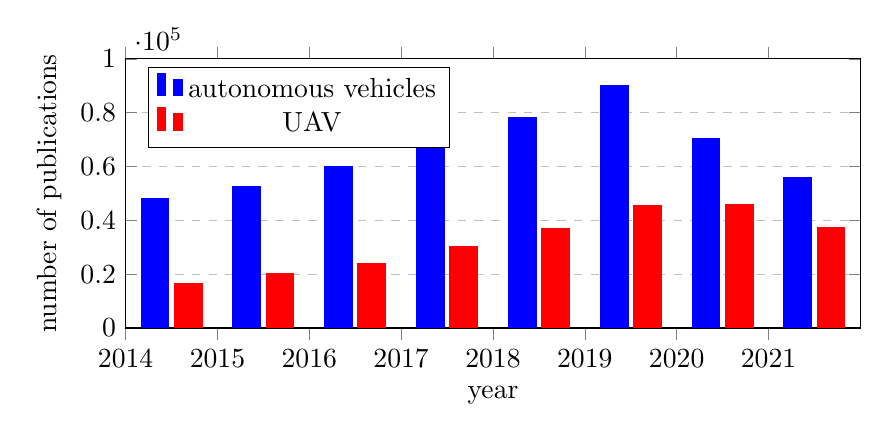
\begin{tikzpicture}
\begin{axis}[
	/pgf/number format/1000 sep={},
	ybar,bar width=10pt,
    xlabel={year},
    ylabel={number of publications},
    xmin=2014, xmax=2022,
    ymin=0, ymax=100000,
    xtick={2012,2013,2014,2015,2016,2017,2018,2019,2020,2021},
    ytick={0,20000,40000,60000,80000,100000,120000},
    legend pos=north west,
    ymajorgrids=true,
    grid style=dashed,
    height=5cm,
    width=0.9\textwidth
    ]

\addplot+[ybar,
    color=blue
    ]
    coordinates {
    (2021.5,55900)
    (2020.5,70300)
    (2019.5,90200)
    (2018.5,78000)
    (2017.5,68100)
    (2016.5,60100)
    (2015.5,52500)
    (2014.5,48200)
    };

\addplot+[ybar,
    color=red
    ]
    coordinates {
    (2021.5,37300)
    (2020.5,46000)
    (2019.5,45400)
    (2018.5,36800)
    (2017.5,30200)
    (2016.5,23900)
    (2015.5,20300)
    (2014.5,16500)
    };
    \legend{autonomous vehicles, UAV}
\end{axis}
\end{tikzpicture}
\caption{Number of released papers with specific keywords per year}
\label{fig:auav}
\end{figure}

\subsection{Fire Detection}

As seen in figure \ref{fig:fd}, fire detection is an interest rich topic with regards to academic production, with a large and steady number of papers throughout the last 10 years. This leads us to believe that this topic continues to interest the scientific community, and we may find interesting and innovative solutions to this problem, as well as tried and tested ones.

\begin{figure}[htb]
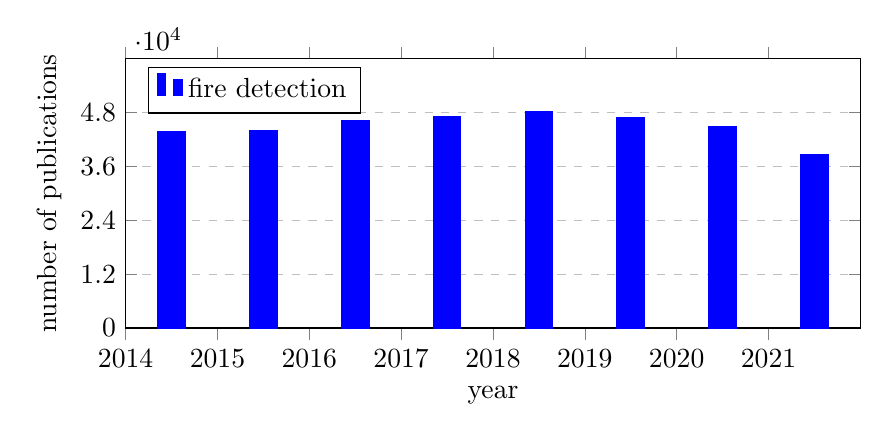
\begin{tikzpicture}
\begin{axis}[
	/pgf/number format/1000 sep={},
	ybar,bar width=10pt,
    xlabel={year},
    ylabel={number of publications},
    xmin=2014, xmax=2022,
    ymin=0, ymax=60000,
    xtick={2012,2013,2014,2015,2016,2017,2018,2019,2020,2021},
    ytick={0,12000,24000,36000,48000},
    legend pos=north west,
    ymajorgrids=true,
    grid style=dashed,
    height=5cm,
    width=0.9\textwidth
    ]

\addplot+[ybar,
    color=blue
    ]
    coordinates {
    (2021.5,38700)
    (2020.5,45000)
    (2019.5,46900)
    (2018.5,48200)
    (2017.5,47200)
    (2016.5,46300)
    (2015.5,44000)
    (2014.5,43900)
    };
    \legend{fire detection}
\end{axis}
\end{tikzpicture}
\caption{Number of released papers with specific keywords per year}
\label{fig:fd}
\end{figure}

\subsection{Fire Suppression}

Academic production for the fire suppression topic has remained somewhat constant through the last 10 years, as can be seen in figure \ref{fig:fs}. From this we can ascertain that although there may not be an increasing number of papers and interest, there is constant interest and paper releases. This leads us to believe that this topic still interests the scientific community, and we may find interesting and innovative solutions to this problem still. 

\begin{figure}[htb]
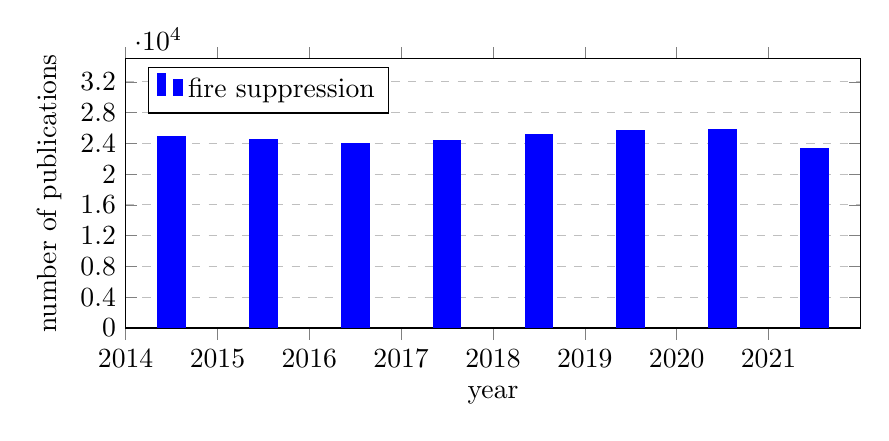
\begin{tikzpicture}
\begin{axis}[
	/pgf/number format/1000 sep={},
	ybar,bar width=10pt,
    xlabel={year},
    ylabel={number of publications},
    xmin=2014, xmax=2022,
    ymin=0, ymax=35000,
    xtick={2012,2013,2014,2015,2016,2017,2018,2019,2020,2021},
    ytick={0,4000,8000,12000,16000,20000,24000,28000,32000},
    legend pos=north west,
    ymajorgrids=true,
    grid style=dashed,
    height=5cm,
    width=0.9\textwidth
    ]

\addplot+[ybar,
    color=blue
    ]
    coordinates {
    (2021.5,23300)
    (2020.5,25800)
    (2019.5,25700)
    (2018.5,25100)
    (2017.5,24400)
    (2016.5,24000)
    (2015.5,24500)
    (2014.5,24900)
    };
    \legend{fire suppression}
\end{axis}
\end{tikzpicture}
\caption{Number of released papers with specific keywords per year}
\label{fig:fs}
\end{figure}

\section{State of the Art}

\subsection{Autonomous \acrshort{uav}}

\acrshort{uav} are a technology with the potential to solve a variety of issues across various industries. The last decade has shown an increased interest and investment in \acrshort{uav} and it's autonomous operation. Has such, a variety of important developments have been made in drone communication, routing, efficiency and applications.

\subsubsection{Energy Consumption}

One of the foremost limiting factors of \acrshort{uav} utilization is their restricted energy capacity and it's management \cite{8255733}. The flight duration of \acrshort{uav} is impacted by their respective battery capacity and payload (including sensors and communication devices) \cite{8579209}.

In order to resolve this factor, energy consumption modelling is used to optimize battery usage and vehicle weight. Such techniques include (but are not limited to):

\begin{itemize}
	\item Empirical model based on energy consumption at variable speeds \cite{inproceedings1}
	\item Heuristic model using \acrfull{milp} which takes into account collision, grounding, fuel efficiency and communication constraints \cite{Grotli2012} 
\end{itemize}

\subsubsection{Route Planning}

Furthermore, we also find the need to effectively and safely route \acrshort{uav} within a given environment, with several factor to take into account: communication, collisions, energy and area restrictions \cite{inproceedings}. In order to solve these issues, solutions have been proposed:

\begin{itemize}
	\item \acrshort{uav} swarm path planning constrained by energy availability \cite{inproceedings}
	\item Edge computing based obstacle avoidance based on linear model predictive controller \cite{inproceedings2}
\end{itemize}

\subsubsection{Communication}

In order for a given \acrshort{uav} based system to be effective, each drone should be able to connect and communicate in a multiple agent network. In order to do this, there exist two solution types: a central unit with which each drone communicates with, and a mesh based network, where each drone communicates with each other. Such solutions include:

\begin{itemize}
	\item Forest fire detection system composed of \acrshort{uav} and ground stations, used for communication and energy management \cite{inproceedings3}
	\item Swarm based \acrshort{uav} telecommunication coverage extender in disaster situations \cite{6318390}
\end{itemize}

\subsubsection{Autonomy}

Autonomy can be divided into two distinct subtopics within \acrshort{uav}: autonomy regarding the ability of an aircraft to perform it's tasks without human operation as well as autonomy with regards to the operation and management of drone clusters without human intervention.

The former task has seen a wide range of innovations using artificial intelligence models to navigate a given environment. Such innovations include:

\begin{itemize}
	\item Real-time model-based reinforcement learning (TEXPLORE) \cite{7838739}
	\item Autonomous navigation using low cost sensors using a error-state Kalman filter (ESKF) \cite{Youn2021}
	\item Path planning using deep reinforcement learning in dynamic environments \cite{ZHANG2022108194}
\end{itemize}

The latter task has seen some innovations with regards to multi-agent systems, whereas each drone acts as an independent operator in the environment and works in cooperative or competitive ways to perform a set of tasks. Such systems include:

\begin{itemize}
	\item Cooperative multi-agent based system with one agent acting as a leader to other agents \cite{10.1007/978-3-030-49778-1_28}
	\item Competitive multi-agent system used to optimize task allocation in a multiple \acrshort{uav} system \cite{inproceedings4}
	\item \acrfull{madrl} centralized and decentralized systems used for cooperative tracking guidance and confrontation \cite{ZHOU2022100} \cite{article23}
\end{itemize}

\subsection{Fire Detection}

\subsection{Fire Suppression}

\section{Applications}

\subsection{Autonomous \acrshort{uav}}

\subsection{Fire Detection}

\subsection{Fire Suppression}

\section{Conclusion}

\bibliography{refs}

\end{document}